\chapter{Metodologia de desenvolvimento}
\label{metodologiaDesenvolvimento}
Este capítulo apresenta a proposta e implementação de um protótipo de rede social para criação e divulgação de vagas em bolsas na universidade e estágios. Inicialmente é realizado um levantamento de requisitos da aplicação. Em seguida, são detalhados a arquitetura e o projeto de banco de dados utilizados como guias para o desenvolvimento da rede social. Na sequência, o processo de implementação do sistema é detalhado, exibindo tomadas de decisões baseadas em padrões de projeto em engenharia de software.

\section{Visão Geral}
\label{metodologiaVisaoGeral}
O objetivo da rede social é apresentar de uma maneira mais centralizada, interativa, intuitiva e organizada listas de vagas disponíveis tanto em bolsas na universidade quanto em estágios dentro e fora do meio acadêmico. Com a centralização de informações, os usuários poderiam através do seu login do INF pesquisar, recomendar e candidatar-se a vagas ofertadas e dados pessoais, profissionais ou acadêmicos, como histórico escolar, solicitados na vaga já seriam encaminhados automaticamente. Ainda, por ser uma rede social, é possível explorar uma maior interação entre os usuários, promovendo um networking e facilitando indicações a vagas futuras.

O ambiente implementado é um protótipo de aplicação Web baseado em uma arquitetura centralizada em dados \cite{pressman}, uma vez que é o padrão mais utilizado na Internet \cite{kurose}. A rede social pode ser acessada por navegadores Web mais modernos que possuem suporte às tecnologias HTML5 e CSS3. Em especial, todos os navegadores mais utilizados atualmente como Google Chrome, Mozilla Firefox, Opera, Safari e Edge.

O desenvolvimento no lado servidor foi realizado utilizando o motor de template Twig para a linguagem PHP, pois fornece recursos que facilitam a implementação de uma arquitetura MVC, além de possuir uma sintaxe que aumenta a legibilidade do código, facilitando sua manutenção. Complementarmente, para a comunicação com o banco de dados, foi utilizado um modelo Entidade-Relacionamento e o banco de dados escolhido foi SGBD relacional MySQL por ser uma ferramenta livre, popular e robusta \cite{mysql}.

O lado do cliente, por sua vez, foi constituído da união das tecnologias HTML5, CSS3, JavaScript e o framework jQuery. Este último é uma biblioteca de funções do JavaScript nativo que facilitam a prototipagem de aplicações e concedem suporte a diferentes tipos de browser, aumentando assim a portabilidade do sistema.


\section{Requisitos}
\label{metodologiaRequisitos}
Os requisitos de um sistema são descrições dos serviços fornecidos pelo sistema e suas restrições operacionais. Esses requisitos refletem as necessidades dos clientes de um sistema que ajuda a resolver a algum problema \cite{sommerville}. Frequentemente os requisitos de software são classificados em requisitos funcionais, que declaram os serviços que o sistema deve oferecer; e requisitos não funcionais, que são as restrições nas funções oferecidas pelo sistema. 

\subsection{Requisitos funcionais}
\label{requisitosRF}
Os requisitos funcionais referem-se sobre o que o sistema deve fornecer, ou seja, suas funções e informações. Preocupam-se com as funcionalidades, serviços e em como o sistema deve reagir em determinadas situações de acordo com entradas recebidas para satisfazer os requisitos do negócio. Abaixo, são listados os requisitos funcionais deste projeto:  

\begin{itemize}
    \item \textbf{RF01:} Para acessar o sistema, o usuário deverá efetuar o processo de login, utilizando um usuário e uma senha.
    
    \item \textbf{RF02:} O sistema deve permitir consultas sobre o banco de usuários, combinando zero ou mais filtros pré-definidos.
    
    \item \textbf{RF03:} O sistema deve permitir consultas sobre o banco de vagas, combinando zero ou mais filtros pré-definidos.
    
    \item \textbf{RF04:} O sistema deve permitir a inserção de novas vagas.
    
    \item \textbf{RF05:} O sistema deve permitir a edição de vagas existentes.
    
    \item \textbf{RF06:} O sistema deve permitir a exclusão lógica de vagas existentes.
    
    \item \textbf{RF07:} O sistema deve permitir a configuração de dados do usuário de acordo com sua preferência.
    
    \item \textbf{RF08:} O sistema deve permitir que um usuário siga ou deixe de seguir outros usuários unilateralmente.
    
    \item \textbf{RF09:} O sistema deve permitir que um usuário bloqueie ou desbloqueie outros usuários unilateralmente.
    
    \item \textbf{RF10:} O sistema deve permitir a inserção de novas postagens.
    
    \item \textbf{RF11:} O sistema deve permitir a edição de uma postagem já existente.
    
    \item \textbf{RF12:} O sistema deve permitir a exclusão lógica de uma postagem já existente.
    
    \item \textbf{RF13:} O sistema deve permitir que um usuário curta ou descurta uma postagem de outro usuário. 
    
    \item \textbf{RF14:} O sistema deve permitir que um usuário recomende outro usuário ou uma vaga.
\end{itemize}

\subsection{Requisitos não funcionais}
\label{requisitosRNF}
Os requisitos não-funcionais são restrições sobre os serviços ou as funções oferecidas pelo sistema. Elas incluem restrições de \textit{timing}, restrições sobre o processo de desenvolvimento e padrões. Os requisitos funcionais aplicam-se, frequentemente, ao sistema como um todo \cite{sommerville}. Em geral não se aplicam às características ou serviços individuais de sistema. Abaixo, são listados os requisitos não funcionais deste projeto:  

\begin{itemize}
    \item \textbf{RNF01:} O sistema deve ser hospedado em um servidor web.

    \item \textbf{RNF02:} Os dados deverão estar armazenados em um banco de dados relacional e centralizado.  

    \item \textbf{RNF03:} O sistema deve ser de fácil utilização.  

    \item \textbf{RNF04:} O sistema deve funcionar corretamente nos principais navegadores web.

    \item \textbf{RNF05:} O sistema deve ter um visual responsivo, possibilitando o uso em aparelhos mobile.

    \item \textbf{RNF06:} O sistema deve possibilitar dois tipos de usuários para acesso à ferramenta: usuários administradores, que terão acesso a todos os módulos do sistema; e usuários comuns, que poderão apenas consultar e recomendar vagas e interagir de maneira limitada com outros usuários.
\end{itemize}

\section{Arquitetura do sistema}
\label{arquiteturaSistema}
O desenvolvimento da rede social foi projetado para ser uma aplicação na web. Foram escolhidas duas arquiteturas diferentes: uma para centralizada em dados para atender às requisições de serviços do lado do servidor; e outra MVC, utilizada para a implementação da lógica e das telas da plataforma.

\subsection{Arquitetura centralizada em dados}
\label{arquiteturaCentralizadaDados}
A figura \ref{dataCenteredArchitecture} ilustra a arquitetura implementada. O ambiente do servidor, por residir em uma aplicação web receberá várias solicitações de usuários ao passo que ocorrem diversas interações no sistema \cite{kurose}, foi adotada uma configuração cliente-servidor (PRESSMAN) onde o banco de dados é centralizado no servidor que hospeda a rede social.

A linguagem de programação utilizada no desenvolvimento desta arquitetura foi o PHP. Esta é amplamente utilizada em páginas da Internet\footnote{\url{https://w3techs.com/technologies/overview/programming_language/all} Acesso em outubro de 2018}~e, mesmo com o advento de tecnologias emergentes como Node.js\footnote{\url{https://insights.stackoverflow.com/survey/2016\#technology} Acesso em outubro de 2018}~, mantém-se firme no mercado especialmente em questões \textit{server-side}. Por ser uma linguagem de código aberto, apresenta uma grande e participativa comunidade que constantemente desenvolve \textit{plugins}, \textit{frameworks} e bibliotecas para atender diversas demandas de desenvolvedores \cite{phpPatternsArticle2016}

\begin{figure}[ht]
    \caption{Arquitetura centralizada em dados.}
       	\begin{center}
            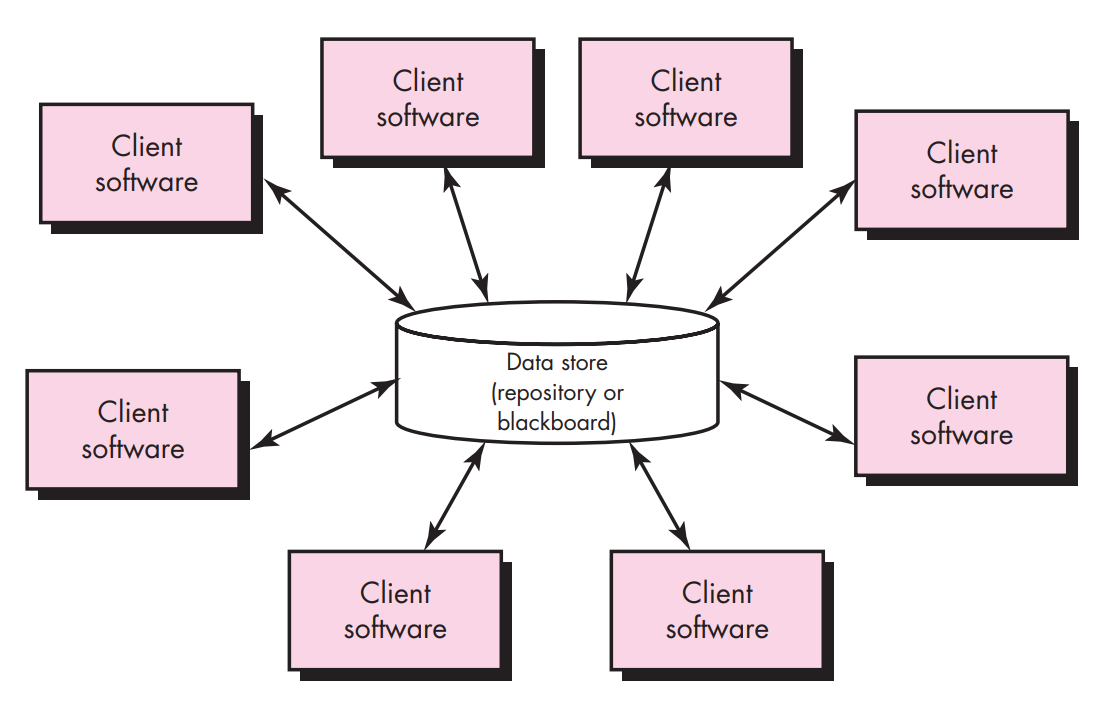
\includegraphics[width=0.68\textwidth]{arquitetura-centralizada-dados.png}
        \end{center}
    \label{dataCenteredArchitecture}
    \legend{Fonte: \cite{pressman}}
\end{figure}

\subsection{Arquitetura MVC}
\label{arquiteturaMVC}

Outra arquitetura de desenvolvimento de software adotada foi o MVC. Esta arquitetura desacopla a lógica da aplicação da interface do usuário, permitindo desenvolver, analisar e testar separadamente cada parte. O modelo engloba todo domínio específico à aplicação e seu processamento lógico como funcionalidades e acesso a dados externos e fontes de informação. A visão é responsável por exibir, na saída de dados, o conteúdo do modelo em um formato legível e requisitado pelo usuário final. O controlador coordena a comunicação entre o modelo e a visão de acordo com as requisições do usuário. A figura \ref{dataMVCArchitecture} ilustra a arquitetura implementada

\begin{figure}[ht]
    \caption{Arquitetura MVC.}
       	\begin{center}
            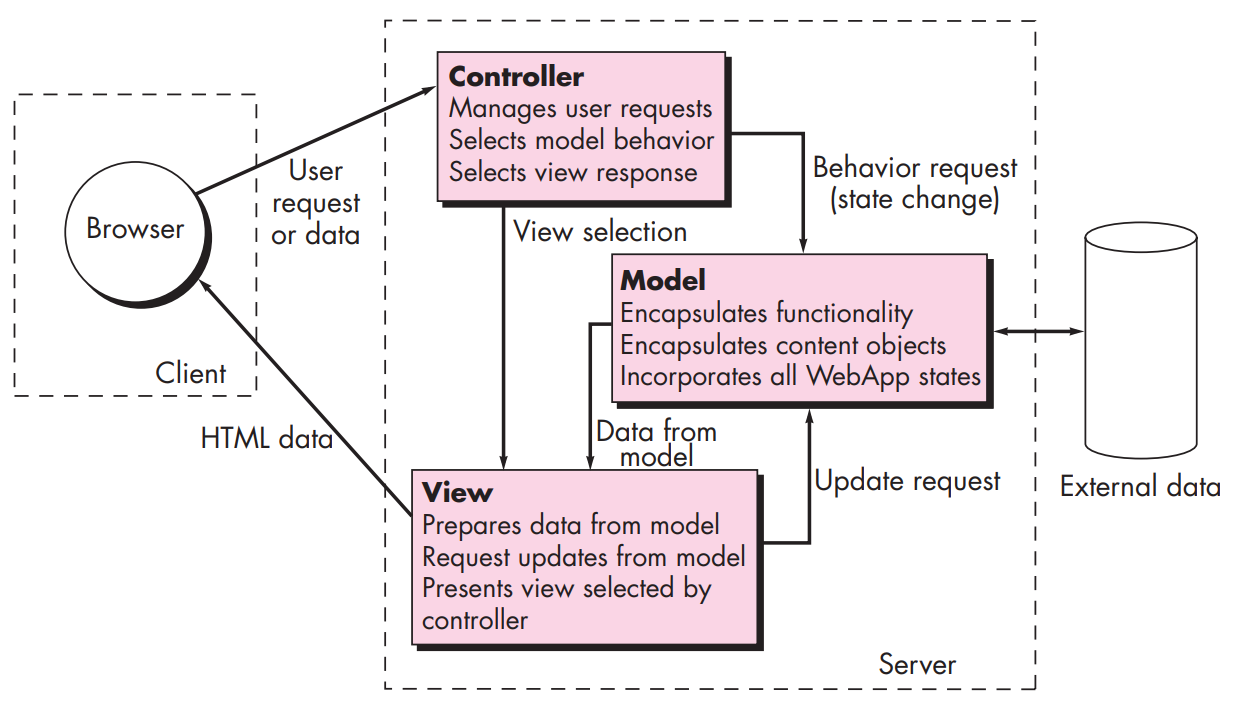
\includegraphics[width=0.68\textwidth]{arquitetura-mvc.png}
        \end{center}
    \label{dataMVCArchitecture}
    \legend{Fonte: \cite{pressman}}
\end{figure}

A arquitetura foi desenvolvida através, novamente, da linguagem de programação PHP. Para auxiliar na abstração e no desacoplamento entre os três módulos da arquitetura MVC, foi utilizado o motor de template Twig\footnote{\url{https://twig.symfony.com/} Acesso em outubro de 2018}. A ferramenta Twig  permite escrever um código mais conciso, com \textit{templates} mais legíveis e amigáveis para \textit{web designers} e, em vários casos, mais poderosos que \textit{templates} padrões do PHP \cite{symfonyBook}.

\begin{figure}[ht]
    \caption{Exemplo de \textit{template} padrão em PHP.}
       	\begin{center}
            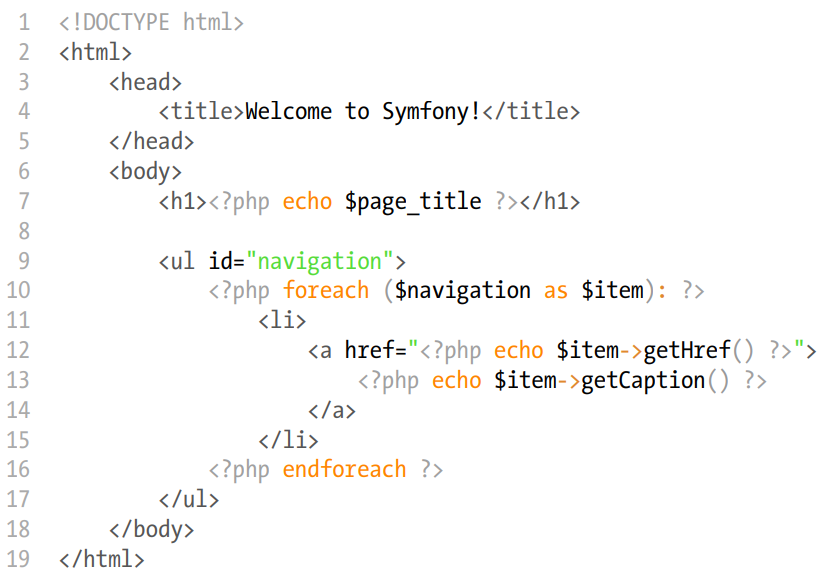
\includegraphics[width=0.68\textwidth]{twig-php.png}
        \end{center}
    \label{codeTemplatePHP}
    \legend{Fonte: \cite{symfonySensioLabs}}
\end{figure}

\bigskip

\begin{figure}[ht]
    \caption{Exemplo de \textit{template} em Twig .}
       	\begin{center}
            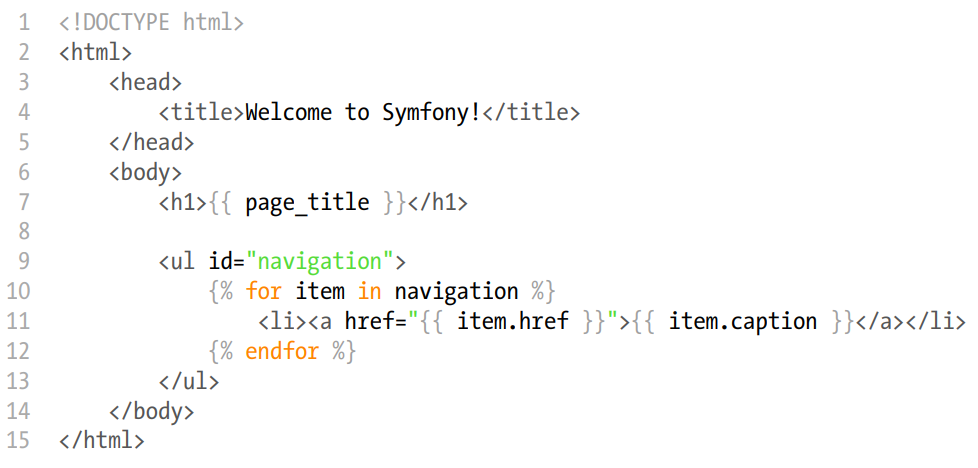
\includegraphics[width=0.68\textwidth]{figuras/twig-symf.png}
        \end{center}
    \label{codeTemplateTwig}
    \legend{Fonte: \cite{symfonySensioLabs}}
\end{figure}


\section{Projeto de Banco de dados}
\label{metodologiaBD}

O banco de dados utilizado na rede social foi o SGBD relacional MySQL. A ferramenta é livre, popular, robusta e amplamente utilizada em aplicações na Internet \footnote{\url{https://db-engines.com/en/ranking} Acesso em outubro de 2018}. O MySQL utiliza a linguagem SQL, \textit{Structured Query Language}, padrão dos bancos de dados relacionais para realizar consultas e atualizar informações nos dados armazenados pelo sistema \cite{sqlCompleteBook}.

O projeto de um banco de dados dá-se em duas fases: a modelagem conceitual, onde é construído um diagrama de entidade-relacionamento \cite{peterChen1976} e são capturadas as necessidades da organização independente de implementação; e o projeto lógico, que objetiva transformar o modelo conceitual em um modelo lógico, isto é, o modo como o banco de dados será implementado em um SGBD específico \cite{heuser}.

\subsection{Modelagem conceitual}
\label{BDModelagem}

A modelagem conceitual é utilizada para obter uma descrição abstrata, independente de implementação em computador, dos dados que serão armazenados no banco de dados. A técnica de modelagem de dados mais difundida e utilizada é a abordagem entidade-relacionamento (ER). \cite{heuser} Através dela, os modelos de dados são representados graficamente por um diagrama entidade-relacionamento (DER). A figura \ref{modelagemBDExemplol} apresenta um DER parcial presente na modelagem conceitual do sistema implementado.

\begin{figure}[h]
    \caption{Exemplo de modelagem conceitual.}
       	\begin{center}
            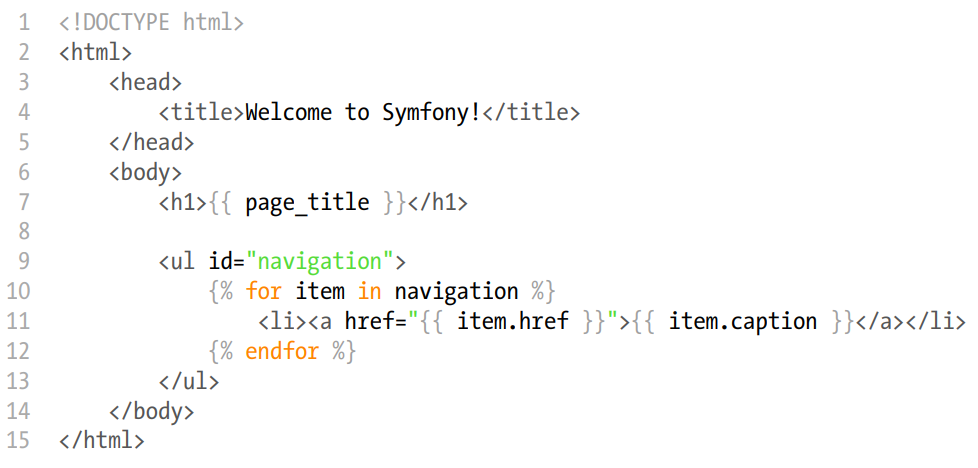
\includegraphics[width=0.68\textwidth]{figuras/twig-symf.png}
        \end{center}
    \label{modelagemBDExemplol}
    %\legend{Fonte: Autor}%
\end{figure}

\subsection{Projeto lógico}
\label{BDProjeto}

O projeto lógico consiste na transformação de um modelo ER em um modelo lógico. Este implementa de forma concreta, a nível de SGBD relacional, os dados representados no modelo ER.

Um determinado modelo ER pode ser implementado através de diversos modelos relacionais, que contém as informações especificadas pelo diagrama ER. Todos podem ser considerados uma implementação correta do modelo ER considerado. Entretanto, diferentes modelos relacionais podem resultar em diferentes performances do sistema construído sobre o banco de dados. 

No processo de transformação do modelo ER para o modelo relacional, foram utilizadas as seguintes regras de transformação \cite{heuser} a fim de obter uma melhor performance do sistema: 

\begin{itemize}
    \item Obter um banco de dados que permita boa performance de instruções de consulta e alteração do banco de dados.
    
    \item Obter um banco de dados que simplifique o desenvolvimento e a manutenção de aplicações.
    
    \item Evitar junções.
    
    \item Diminuir o número de chaves primárias.
    
    \item Evitar campos opcionais.
    
\end{itemize}

Os dois primeiros itens são alcançados naturalmente com as funcionalidades nativas do SGBD MySQL \cite{sqlCompleteBook}. As junções só ocorrem quando há uma relação 1:N entre duas entidades diferentes no sistema, minizando a quantidade de uso e consequente impacto dessas operações. Por fim, os dois últimos itens são respeitados com uma padronização de tabelas feitas para o projeto: todas possuem chave primária única e nenhum campo opcional. A figura \ref{modelagemBDLogicoExemplol} apresenta a transformação do modelo ER para o modelo relacional do exemplo apresentado na figura \ref{modelagemBDExemplol}.

\begin{figure}[h]
    \caption{Exemplo de modelagem relacional.}
       	\begin{center}
            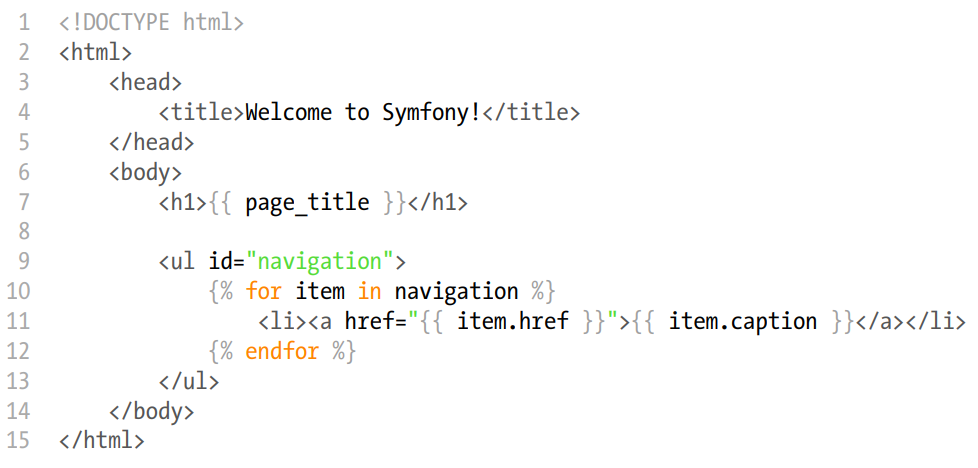
\includegraphics[width=0.68\textwidth]{figuras/twig-symf.png}
        \end{center}
    \label{modelagemBDLogicoExemplol}
    %\legend{Fonte: Autor}%
\end{figure}

\subsection{Criação do banco de dados}
\label{BDCriacao}

A etapa final do projeto de banco de dados consiste na implementação do modelo lógico de acordo com as regras e definições do SGBD escolhido. Para a transcrição do modelo em tabelas MySQL, foi utilizado o módulo do phpmyadmin que faz parte dos softwares e recursos instalados junto à pilha XAMPP (ver seção \ref{implementacaoConfig}). Através dessa ferramenta, é possível realizar consultas e  operações no SGBD como criação, edição e remoção de tabelas e registros.

\begin{figure}[h]
    \begin{adjustwidth}{-1in}{-.8in}
        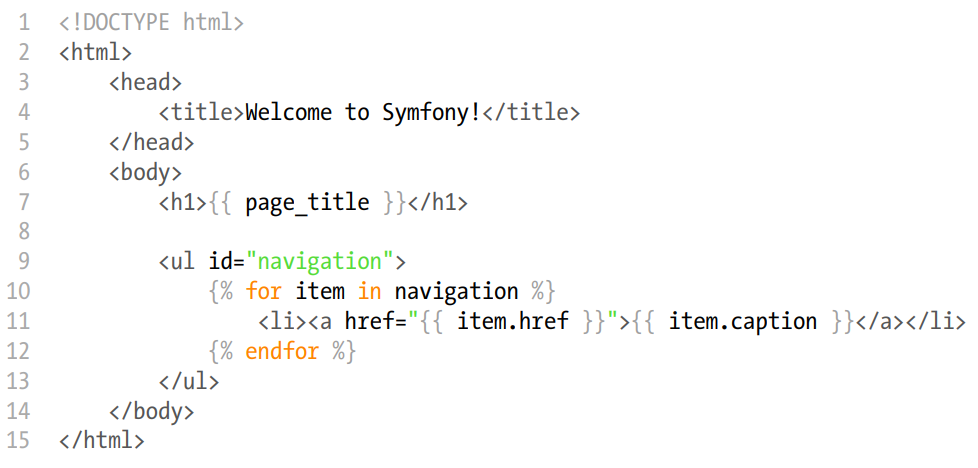
\includegraphics[width=0.68\textwidth]{figuras/twig-symf.png}
        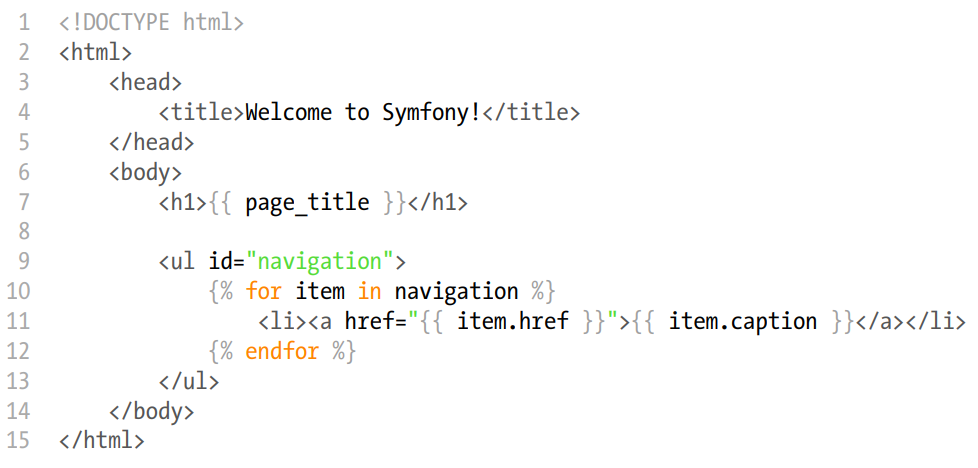
\includegraphics[width=0.68\textwidth]{figuras/twig-symf.png}
        \caption{Telas para criação do banco de dados e configuração da tabela [nome tabela].}
        \label{projetoImagens}
    \end{adjustwidth}
\end{figure}

Ao final deste processo, a implementação do banco de dados da rede social foi concluído com 17 tabelas, sendo elas:

\begin{itemize}
    \item \textbf{block:} registra uma ação de bloqueio entre dois usuários, representado pelo campo "id\_blocker", correspondente ao usuário bloqueante, e "id\_blocked", usuário bloqueado. São armazenadas ainda a informação de quando ocorreu a ação pelo campo "datetime\_created"\ e se o bloqueio está ativo ainda, visto que é uma ação reversível, através do campo "active".
    
    \item \textbf{comment:} tabela que gerencie os comentários em postagens de usuários. Composta pelos campos "id\_author", que é o \textit{id} do usuário que fez o comentário; "id\_post", \textit{id} da postagem onde foi feito o comentário; "text", o conteúdo propriamente do comentário; "datetime\_published"\ e "datetime\_last\_edit"\ correspondem às datas de postagem e última edição respectivamente; "active", indica se o comentário está visível ou não (excluído).
    
    \item \textbf{favorite:} 
    
    \item \textbf{follow:} registra uma ação de seguir entre dois usuários, representado pelo campo "id\_follower", correspondente ao usuário seguidor, e "id\_following", usuário seguido. São armazenadas ainda a informação de quando ocorreu a ação pelo campo "datetime\_created"\ e se o ato de seguir está ativo ainda, visto que é uma ação reversível, através do campo "active".
    
    \item \textbf{job:} representa uma vaga divulgada no sistema. "id\_author"\ guarda o \textit{id} do usuário que criou a vaga; "title"\ é o título da vaga; "category\_list"\ é uma lista de \textit{id} de categorias da tabela \textit{job\_category} que determinam as áreas de atuação da vaga; "resume"\ é uma descrição breve da vaga ofertada e "text", o texto completo; "skills"\ é a lista de habilidades que são interessantes o candidato possuir; "type"\ é o tipo de vaga ofertada: pode ser 0 para Monitoria, 1 para Bolsa administrativa, 2 para Bolsa de iniciação científica, 3 para Estágio, 4 para Trainee, 5 para Efetivo ou 6 para Voluntário; "modality"\ é a modalidade da vaga: 0 corresponde a uma vaga Presencial, 1 À distancia; "salary"\ representa a remuneração mensal; "semester"\ indica a partir de qual semestre o candidato estaria apto para se candidatar; "shift"\ registra em qual(is)  turno(s) o candidato terá de trabalhar, "is\_prae"\ é um campo booleano e representa se a vaga, caso seja uma bolsa da UFRGS, é exclusiva para beneficiários PRAE ou não; os campos "date\_start"\ e "date\_finish"\ indicam o período de vigência da vaga; "workload"\ corresponde ao total de horas semanais a vaga exige do candidato; os campos "location", "location\_city"\ e "location\_state" determinam o endereço da vaga; "need\_curriculum" especifica se a vaga exige \textit{curriculum vitae} do candidato; "need\_historic", de maneira semelhante, especifica se a vaga exige histórico escolhar do candidato; "datetime\_publication"\ e "datetime\_last\_edit"\ sinalizam as datas e horários que a vaga foi publicada e editada pela última vez respectivamente; por fim, o campo "active"\ guarda a informação se a vaga está disponível ou foi excluída.
    
    \item \textbf{job\_apply:} armazena informações quando um usuário manifesta interesse por uma vaga. O campo "id\_user" guarda o \textit{id} do usuário que realizou a ação e "id\_job", o \textit{id} da vaga em si. Adicionalmente, o campo "datetime\_created"\ registra a data e horário da ação e a coluna "active"\ indica se a manifestação de interesse está ativa ainda, pois o usuário pode desfazer sua ação.
    
    \item \textbf{job\_category:} essa tabela corresponde às áreas de atuação relacionadas a uma vaga. O campo "id" é utilizado como chave estrangeira para a lista presente em "category\_list" da tabela \textit{job}. 
    
    \item \textbf{log:}
    
    \item \textbf{post:} armazena todas as informações de um post feito por um usuário. O campo "id\_author" indica o \textit{id} do usuário que fez a postagem; "text" é o conteúdo da postagem; "datetime\_published"\ e "datetime\_last\_edit" representam as datas de criação e última edição da postagem respectivamente; "privacy"\ restringe a exibição do \textit{post}: 1, somente o autor pode olhar ou 0, todos os usuários; "allow\_comments"\ caso possua o valor 1, qualquer usuário pode comentar na postagem, caso contrário, nenhum pode; "active" é um indicativo se o post está visível ou não (foi excluído pelo autor).
    
    \item \textbf{post\_like:} registra a curtida de um usuário em um post. Os campos criados para a tabela são: "id\_user", referente ao \textit{id} do usuário; "id\_post", que diz respeito ao \textit{id} do post; "datetime\_created"\ informa a data e horário que ocorreu a ação do usuário; "active"\ sinaliza se a curtida está ativa, uma vez que a ação pode ser desfeita.
    
    \item \textbf{recommendation\_job:}
    \item \textbf{recommendation\_user:}
    
    \item \textbf{user:} tabela que salva todos os dados do usuário no sistema. É composta por x campos, sendo eles: "name"\ representa o nome do usuário no sistema; "age"\ é a idade do usuário; "born\_in\_city"\ e "born\_in\_state"\ indicam a cidade e o estado do local de nascimento respectivamente; "live\_in\_city"\ e "live\_in\_state"\ indicam a cidade e o estado onde o usuário reside no momento. "role"\ é a função deste no sistema sendo o valor 1 para Administrador; 2, professor; 3, técnico; 4, aluno. "phone"\ é o seu telefone de contato principal; "birthday"\ sua data de nascimento; "gender", seu sexo onde 0 é Masculino e 1, Feminino; "personal\_link" é um campo para o usuário divulgar sua página pessoal através de um link na Internet; "avatar"\ guarda o caminho relativo da imagem utilizada como foto de perfil do usuário no sistema; "email\_notification"\ sinaliza a preferência do usuário para receber e-mails de notificação do sistema; "show\_schollar\_info"\ e "show\_curriculum"\ são campos que, caso o usuário deseje, ele pode exibir as informações de histórico escolar e currículo no seu perfil respectivamente (valor 1 na coluna) ou omiti-los (valor 0); os campos "follower\_privacy"\ e "following\_privacy"\ restringem o acesso a informações sobre quem o usuário segue e quem o segue para usuários que não o seguem; "post\_privacy"\ é uma comodidade do sistema: indica a opção padrão durante criação de postagens; "datetime\_joined"\ salva a data de ingresso da primeira vez que o usuário fez \textit{login} no sistema. Este último e ainda os campos "id", "login", "email", "password" tiveram de ser simulados devido a restrições de integração do sistema (Ver seção \ref{redeLimitacao}).
    
    \item \textbf{user\_education:} relaciona um qualificação de ensino a um usuário. O campo "id\_user"\ é a chave estrangeira para o \textit{id} de um usuário na tabela \textit{user}. As colunas "title"\ e "subtitle"\ se referem ao grau de instrução ou informação de curso e a escola, universidade ou outra instituição de ensino onde o usuário estudou. "date\_start"\ e "date\_finish"\ guardam as informações do período que o usuário estudou na instituição. "location\_city"\ e "location\_state"\ mostram a cidade e o estado do ensino. O campo "selected"\ sinaliza se o trabalho é destaque; cada usuário pode destacar apenas um trabalho para ser exibida em informações simplificadas de perfil. Ainda, "active"\ informa se o dado está ativo ou foi excluído.
    
    \item \textbf{user\_job:} relaciona uma experiência de trabalho a um usuário. O campo "id\_user"\ é a chave estrangeira para o \textit{id} de um usuário na tabela \textit{user}. As colunas "title"\ e "company"\ se referem ao cargo e empresa onde o  usuário trabalhou. "date\_start"\ e "date\_finish"\ guardam as informações do período que o usuário trabalhou na empresa. "location\_city"\ e "location\_state"\ mostram a cidade e o estado do trabalho. A coluna "selected"\ sinaliza se o trabalho é destaque; cada usuário pode destacar apenas um trabalho para ser exibida em informações simplificadas de perfil. Por fim, "active"\ informa se o registro está ativo ou foi excluído.
    
    o idioma em questão. "level" indica o nível que o usuário possui, sendo 1 para Básico; 2, Intermediário; 3, Avançado; 4, Fluente; 5, Nativo. A coluna "active" informa se o dado está ativo ou foi excluído pelo usuário.
    
    \item \textbf{user\_language:} representa o conhecimento de um usuário sobre uma língua. O campo "title"\ é o idioma em questão. "level" indica o nível que o usuário possui, sendo 1 para Básico; 2, Intermediário; 3, Avançado; 4, Fluente; 5, Nativo. A coluna "active" informa se o dado está ativo ou foi excluído pelo usuário.
    
    \item \textbf{user\_skill:} representa o conhecimento de um usuário sobre uma língua. O campo "title"\ é o idioma em questão. "level" indica o nível que o usuário possui, sendo 1 para Iniciante; 2, Amador; 3, Júnior; 4, Pleno; 5, Sênior. "time" indica o tempo em anos que o usuário possui com essa habilidade. A coluna "active" informa se o dado está ativo ou foi excluído pelo usuário.
    
\end{itemize}

\section{Implementação}
\label{metodologiaImplementação}

A ferramenta foi implementada utilizando os conceitos de metodologia ágil de desenvolvimento, em especial, o SCRUM. O desenvolvimento da aplicação foi dividido em cinco fases: construção do \textit{framework} e  as entregas Inicial, Alfa, Beta e Final. Para uma maior organização durante toda a realização deste projeto, foi criado um repositório no GitHub\footnote{\url{https://github.com/jaflesch/tcc-ufrgs} Acesso em novembro de 2018} e definidas várias \textit{issues}, que agrupadas em \textit{milestones}, representavam um \textit{sprint}, uma etapa de desenvolvimento específico.

\subsection{Configuração do ambiente do trabalho}
\label{implementacaoConfig}

A construção do \textit{framework} focava em implementar conceitos abstratos da linguagem, arquitetura do sistema e funcionalidades básicas que seriam reaproveitadas nas etapas seguintes, como roteamento das páginas, configuração da conexão ao banco de dados e métodos genéricos.


\subsection{SCRUM}
\label{implementacaoSCRUM}

\subsection{Versão Inicial}
\label{implementacaoIR}

A entrega inicial priorizou a elaboração das principais telas do sistema, como a página Home, Feed de usuários, Vaga, Pesquisa e Login. A funcionalidade de realizar autenticação no sistema também foi implementada nesta etapa junto com consultas ao banco de dados que exibiam informações parciais de entidades como usuário e vaga.

\subsection{Versão Alfa}
\label{implementacaoAR}

A segunda etapa destinou-se à interação entre os usuários. Ao terminar da entrega alfa, já era possível seguir ou deixar de seguir um usuário, bloquear ou desbloquear um usuário, curtir ou descurtir um post e suas curtidas eram contabilizados dinamicamente, favoritar ou desfavoritar vaga, recomendar um usuário ou vaga. 

Sobre os aspectos visuais, foram desenvolvidas as páginas restantes: Configurações Gerais, Configurações de Privacidade, Usuários bloqueados, Seguidores; a barra de menu lateral ficou funcional e com animações ao abrir e fechar. Melhorias na experiência de usuário foram aplicadas com o aumento da área de clique em botões e no uso de cores mais contrastantes.

\subsection{Versão Beta}
\label{implementacaoBR}

A entrega Beta trouxe diversas melhorias às funcionalidades desenvolvidas. A pesquisa de vagas e de usuários ganharam novos filtros de modo a tornar a sua utilização mais inteligente, dinâmica e eficiente. Além disso, a interação quando um usuário manifestava interesse por vaga e a posterior gerência por parte de quem a divulgou foi finalizada. Por fim, a biblioteca de envio de e-mails para registrar e notificar ações importantes realizadas por usuários no sistema foi implementada.

No \textit{frontend}, iniciaram-se os primeiros passos para tratar as questões de responsividade em aparelhos móveis.

\subsection{Versão Final}
\label{implementacaoFR}

documentação e visual
aperfeiçoamento e otimização de funcionalidades